\documentclass[10pt,a4paper]{article}

\usepackage[utf8]{inputenc}
\usepackage[T1]{fontenc}
\usepackage[spanish,es-nodecimaldot]{babel}
\usepackage[top=1.5cm,bottom=2cm,left=1.5cm,right=1.5cm]{geometry}
\usepackage{setspace}
\singlespacing
\usepackage{graphicx}
\usepackage{float}
\usepackage{booktabs}
\usepackage{tabularx}
\usepackage{array}
\usepackage{hyperref}
\usepackage{xcolor}
\usepackage{amsmath}
\usepackage{caption}
\usepackage{parskip}
\usepackage{fancyhdr}

\definecolor{headerdark}{HTML}{2C3E50}
\hypersetup{
  colorlinks=true,
  linkcolor=headerdark,
  citecolor=headerdark,
  urlcolor=blue!70!black,
  pdftitle={Análisis de Enfermedad Cardíaca mediante Técnicas de Data Science},
  pdfauthor={Juan Muñoz, Vicente Rivera, Fernando Valdés}
}

\captionsetup{font=small,labelfont=bf}
\setlength{\parskip}{3pt}
\setlength{\textfloatsep}{8pt plus 1pt minus 2pt}
\setlength{\floatsep}{6pt plus 1pt minus 2pt}
\renewcommand{\arraystretch}{0.95}

\begin{document}

\begin{center}
  {\LARGE \textbf{Análisis de Enfermedad Cardíaca}} \\[3pt]
  {\LARGE \textbf{Clasificación y Clustering en Python}} \\[8pt]
  {\normalsize Juan Muñoz, Vicente Rivera, Fernando Valdés} \\[2pt]
  {\small juan.munozveloso2023@alu.uct.cl, vrivera2023@alu.uct.cl, fvaldes2023@alu.uct.cl} \\[2pt]
  {\small Tarea 5, INFO1184, Semestre I-2026}
\end{center}

\section*{Resumen}

Este informe analiza un conjunto de datos de enfermedad cardíaca disponible en Kaggle, compuesto originalmente por 1.025 registros y 14 variables clínicas y demográficas. El objetivo fue identificar patrones asociados a la presencia de enfermedad cardíaca y evaluar si modelos simples de clasificación permiten detectar pacientes con posible condición cardiovascular. El trabajo se desarrolló en Python siguiendo la metodología CRISP-DM: comprensión del problema, comprensión de datos, preparación, modelamiento y evaluación. Durante la limpieza se detectaron 723 duplicados exactos, por lo que el modelamiento se realizó con 302 registros únicos para reducir sesgo por repetición. El análisis exploratorio mostró que angina inducida por ejercicio, tipo de dolor torácico, depresión ST, frecuencia cardíaca máxima y número de vasos coloreados presentan las asociaciones más fuertes con la variable objetivo. Se compararon regresión logística, K vecinos más cercanos y árbol de decisión; el mejor desempeño fue KNN con accuracy de 0,803 y F1-score de 0,835. Además, K-Means identificó dos perfiles clínicos diferenciados. Los resultados son exploratorios y no constituyen diagnóstico médico.

\textbf{Palabras clave:} enfermedad cardíaca, clasificación, K-Means, CRISP-DM, Python, salud.

\section{Introducción}

La analítica de datos en salud permite transformar registros clínicos en evidencia útil para comprender factores asociados a distintas condiciones médicas. En enfermedades cardiovasculares, variables como edad, presión arterial, colesterol, frecuencia cardíaca, angina inducida por ejercicio y resultados de pruebas clínicas pueden aportar señales relevantes para estudiar riesgo o presencia de enfermedad. No obstante, un modelo construido con fines académicos debe interpretarse con prudencia, ya que no reemplaza evaluación médica ni protocolos clínicos.

El caso de estudio corresponde al \textit{Heart Disease Dataset}, publicado en Kaggle por John Smith \cite{smithkaggle}. La pregunta principal del grupo fue: ¿qué variables clínicas y demográficas se relacionan más con la presencia de enfermedad cardíaca en los pacientes del dataset? A partir de ella se plantearon preguntas secundarias sobre diferencias entre pacientes con y sin enfermedad, capacidad predictiva de modelos simples y posibilidad de identificar perfiles mediante clustering.

El objetivo general fue analizar el dataset mediante análisis exploratorio, visualización, clasificación y agrupamiento. El desarrollo se implementó en ambiente Python, usando un script reproducible y salidas exportadas como evidencia.

\section{Fundamentos de Teoría}

La metodología CRISP-DM organiza proyectos de minería de datos en seis fases: comprensión del negocio, comprensión de los datos, preparación, modelamiento, evaluación y despliegue \cite{chapman2000}. En esta tarea se desarrollaron las primeras cinco fases, porque el alcance solicitado es analítico y no considera implementación productiva.

Para clasificación supervisada se usaron tres modelos de referencia. La regresión logística estima la probabilidad de pertenecer a una clase binaria mediante una función logística aplicada a una combinación lineal de variables \cite{hosmer2013}. K-Nearest Neighbors clasifica una observación según la clase predominante entre sus vecinos más cercanos en el espacio de variables, por lo que requiere escalamiento cuando las magnitudes son distintas \cite{james2021}. El árbol de decisión separa datos mediante reglas sucesivas, facilitando interpretación, aunque puede sobreajustar si no se controla su profundidad \cite{breiman1984}.

El desempeño se evaluó con accuracy, precision, recall y F1-score. Para un problema binario, estas métricas se definen desde verdaderos positivos (VP), falsos positivos (FP), verdaderos negativos (VN) y falsos negativos (FN):

\begin{equation}
  \text{Accuracy}=\frac{VP+VN}{VP+VN+FP+FN}, \quad
  \text{Precision}=\frac{VP}{VP+FP}, \quad
  \text{Recall}=\frac{VP}{VP+FN}.
\end{equation}

\begin{equation}
  F1 = 2 \cdot \frac{\text{Precision}\cdot\text{Recall}}{\text{Precision}+\text{Recall}}.
\end{equation}

Para segmentación no supervisada se aplicó K-Means, algoritmo que particiona observaciones en $k$ grupos minimizando la suma de cuadrados intra-cluster \cite{macqueen1967}. Como apoyo visual se usó PCA para proyectar los clusters en dos dimensiones, manteniendo la interpretación como visualización y no como diagnóstico clínico.

\section{Desarrollo del Trabajo}

\subsection{Comprensión y preparación de datos}

El dataset contiene 14 variables: edad, sexo, tipo de dolor torácico, presión arterial en reposo, colesterol, glucosa en ayunas, electrocardiograma en reposo, frecuencia cardíaca máxima, angina inducida por ejercicio, depresión ST, pendiente ST, vasos coloreados, resultado \textit{thal} y la variable objetivo \texttt{target}. La clase 0 indica ausencia de enfermedad cardíaca y la clase 1 indica presencia.

La revisión inicial identificó 1.025 filas, 14 columnas, cero valores faltantes y 723 duplicados exactos. Dado que registros repetidos pueden inflar artificialmente el rendimiento de modelos, el análisis inferencial y predictivo se realizó sobre 302 registros únicos. La Tabla \ref{tab:limpieza} resume esta etapa.

\begin{table}[H]
\centering
\caption{Resumen de limpieza del dataset.}
\label{tab:limpieza}
\begin{tabular}{lr}
\toprule
Indicador & Valor \\
\midrule
Filas originales & 1.025 \\
Columnas originales & 14 \\
Valores faltantes & 0 \\
Duplicados exactos & 723 \\
Filas luego de eliminar duplicados & 302 \\
Filas removidas & 70,54\% \\
\bottomrule
\end{tabular}
\end{table}

\subsection{Análisis exploratorio}

En el dataset depurado, la clase se mantiene relativamente balanceada: 138 pacientes sin enfermedad y 164 con enfermedad. La Figura \ref{fig:target} muestra esta distribución. Al comparar variables numéricas por clase, los pacientes con \texttt{target=1} presentan menor edad media (52,59 frente a 56,60), menor presión arterial media (129,25 frente a 134,40), colesterol medio ligeramente menor (242,64 frente a 251,09), mayor frecuencia cardíaca máxima (158,38 frente a 139,10) y menor \texttt{oldpeak} medio (0,59 frente a 1,59). Estas diferencias no deben leerse de manera aislada, pues varias variables clínicas son codificadas y la relación puede ser multivariada.

\begin{figure}[H]
\centering
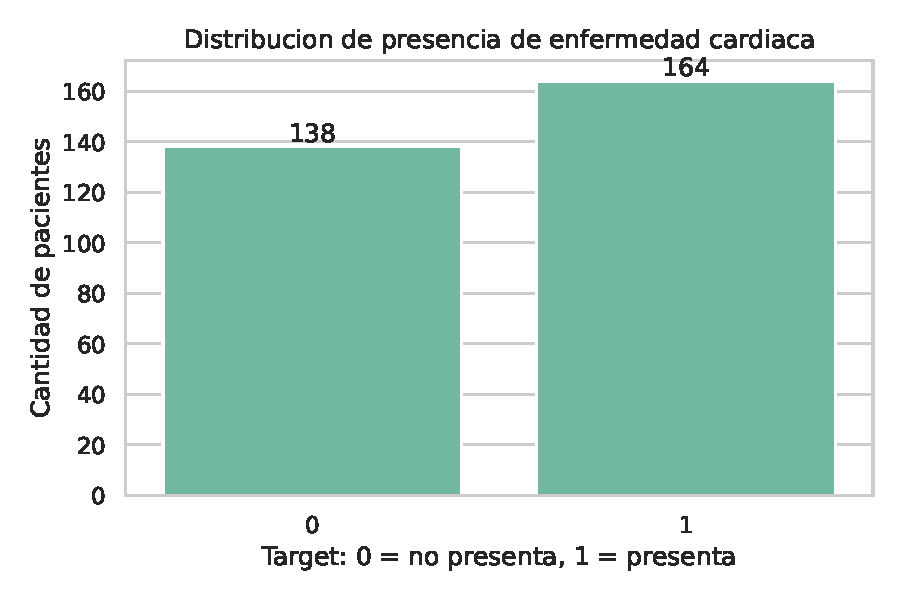
\includegraphics[width=0.58\textwidth]{figuras/fig_01_distribucion_target.pdf}
\caption{Distribución de la variable objetivo en el dataset depurado.}
\label{fig:target}
\end{figure}

\begin{figure}[H]
\centering
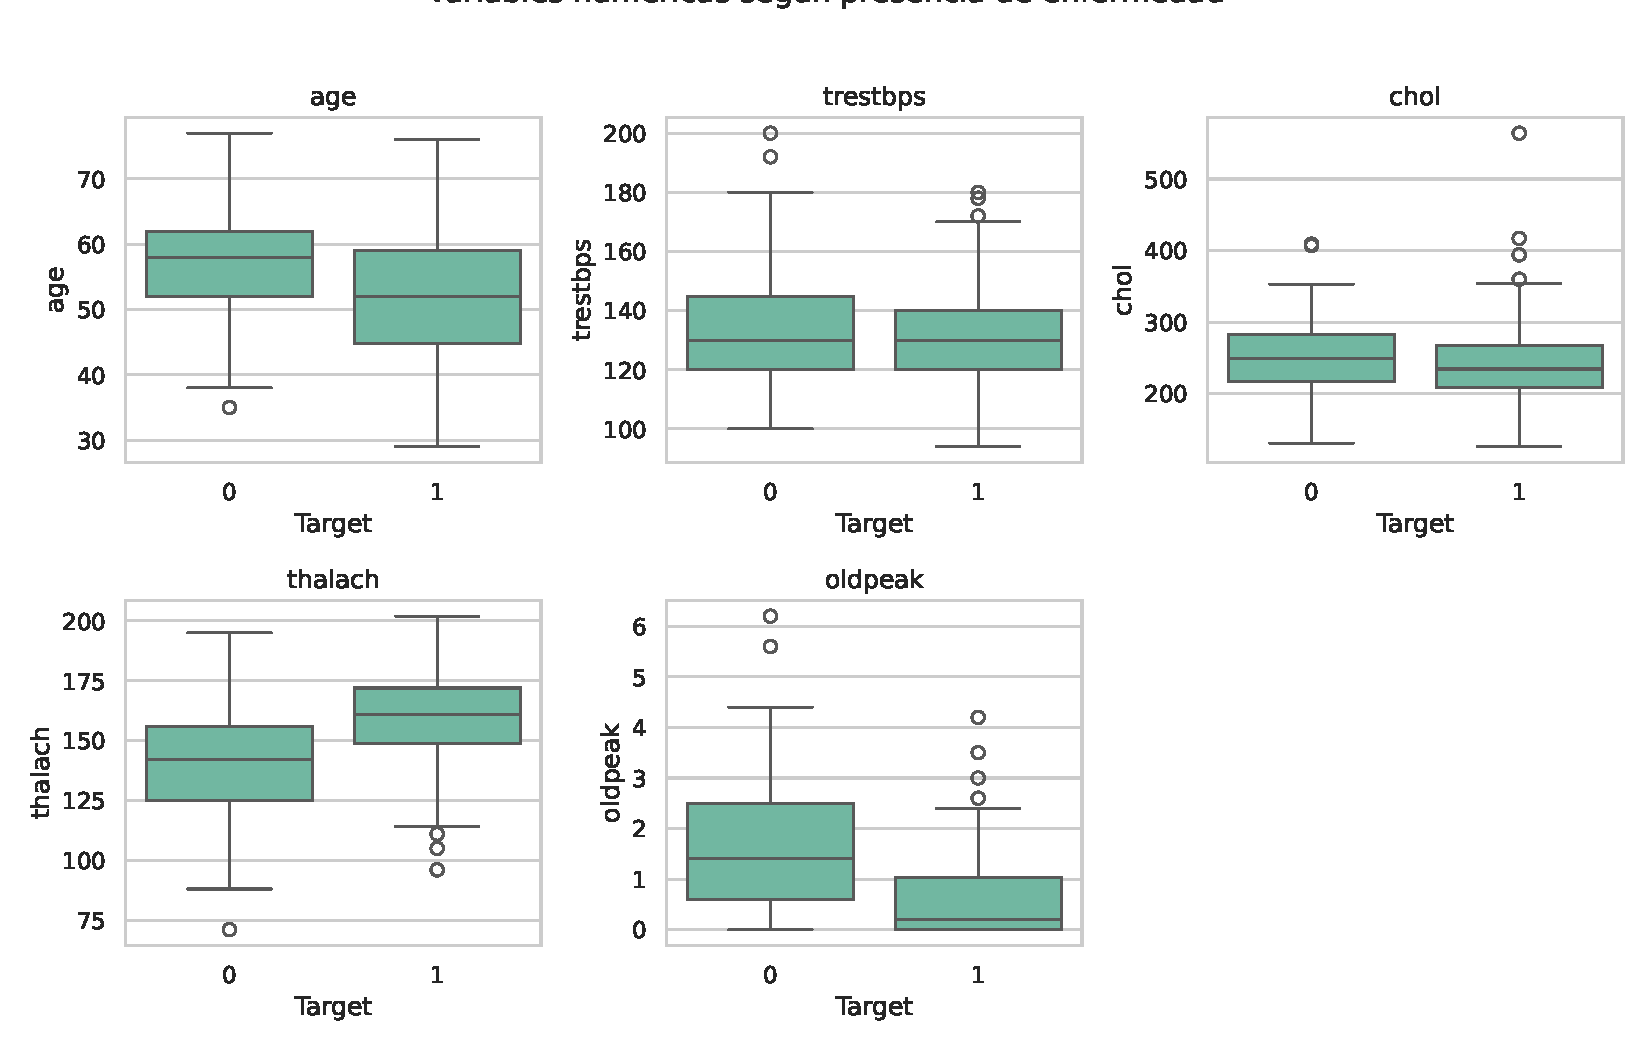
\includegraphics[width=0.9\textwidth]{figuras/fig_02_variables_numericas_por_target.pdf}
\caption{Comparación de variables numéricas según presencia de enfermedad cardíaca.}
\label{fig:numericas}
\end{figure}

La matriz de correlaciones y el ordenamiento por asociación absoluta con \texttt{target} muestran que las variables más relacionadas fueron \texttt{exang} ($r=-0,436$), \texttt{cp} ($r=0,432$), \texttt{oldpeak} ($r=-0,429$), \texttt{thalach} ($r=0,420$) y \texttt{ca} ($r=-0,409$). En contraste, colesterol y glucosa en ayunas presentaron asociaciones lineales bajas en este conjunto depurado.

\begin{figure}[H]
\centering
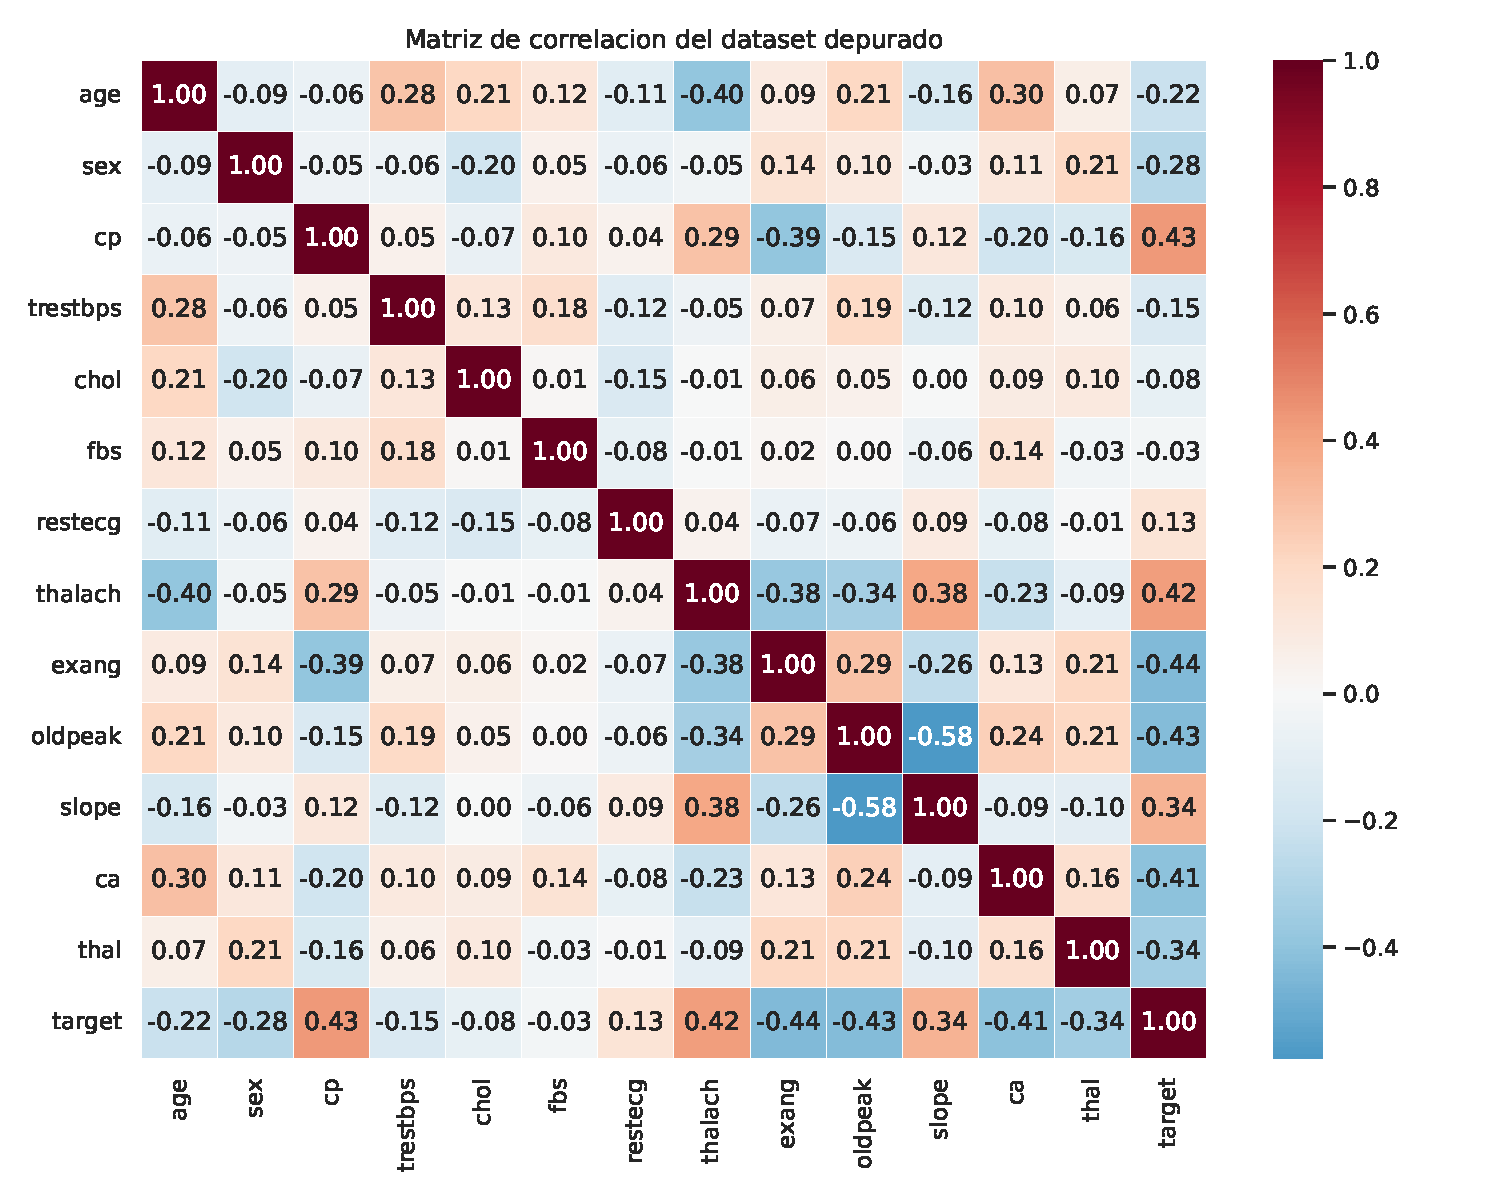
\includegraphics[width=0.82\textwidth]{figuras/fig_03_matriz_correlacion.pdf}
\caption{Matriz de correlación de variables del dataset depurado.}
\label{fig:correlacion}
\end{figure}

\subsection{Clasificación}

Se dividieron los datos en entrenamiento y prueba, usando 25\% para prueba con partición estratificada. Las variables fueron escaladas en regresión logística y KNN. En árbol de decisión se fijó una profundidad máxima de 4 para limitar sobreajuste. La Tabla \ref{tab:modelos} compara los resultados.

\begin{table}[H]
\centering
\caption{Métricas de clasificación en conjunto de prueba.}
\label{tab:modelos}
\begin{tabular}{lrrrr}
\toprule
Modelo & Accuracy & Precision & Recall & F1-score \\
\midrule
KNN k=7 & 0,803 & 0,760 & 0,927 & 0,835 \\
Regresión logística & 0,803 & 0,783 & 0,878 & 0,828 \\
Árbol de decisión & 0,789 & 0,778 & 0,854 & 0,814 \\
\bottomrule
\end{tabular}
\end{table}

El mejor modelo por F1-score fue KNN con $F1=0,835$. Su matriz de confusión obtuvo 23 verdaderos negativos, 38 verdaderos positivos, 12 falsos positivos y 3 falsos negativos. En una aplicación de tamizaje, reducir falsos negativos puede ser valioso, aunque el costo de falsos positivos también debe analizarse clínicamente.

\begin{figure}[H]
\centering
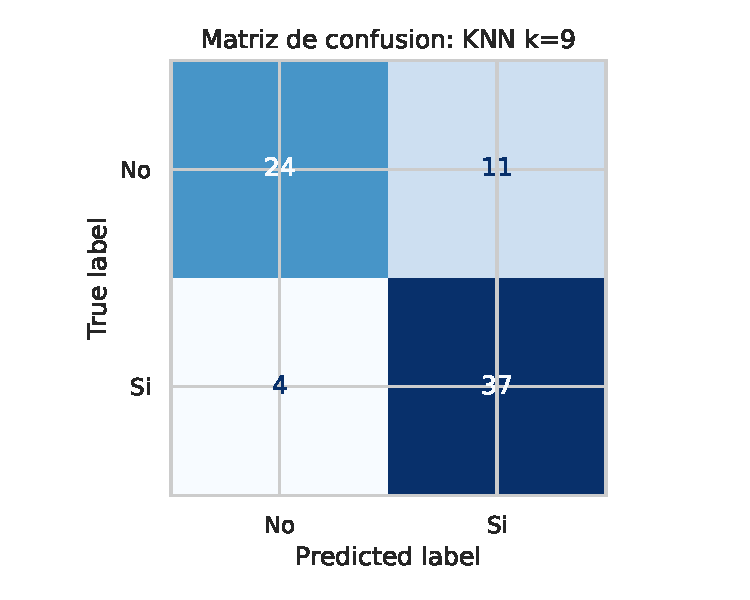
\includegraphics[width=0.55\textwidth]{figuras/fig_05_matriz_confusion_mejor_modelo.pdf}
\caption{Matriz de confusión del mejor modelo de clasificación.}
\label{fig:confusion}
\end{figure}

\subsection{Clustering}

Para clustering se aplicó K-Means sobre las variables predictoras escaladas, sin usar \texttt{target} como entrada. Se evaluaron valores de $k$ entre 2 y 8 mediante inercia y coeficiente de silueta. El mejor valor de silueta fue $k=2$, aunque el valor fue bajo (0,168), lo que sugiere grupos parcialmente solapados y no completamente separados.

\begin{figure}[H]
\centering
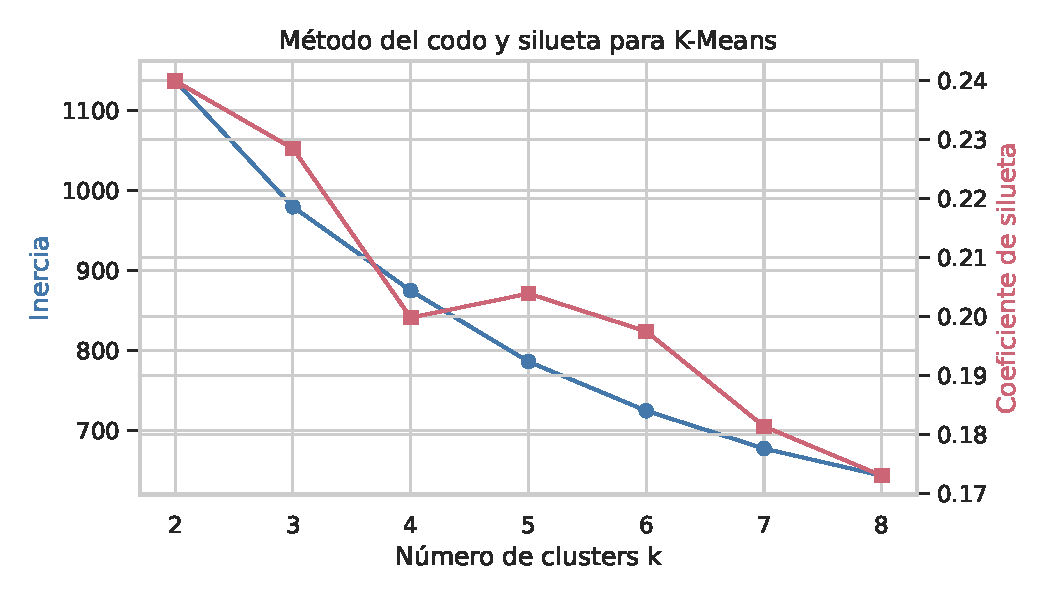
\includegraphics[width=0.72\textwidth]{figuras/fig_07_elbow_kmeans.pdf}
\caption{Método del codo y silueta para selección de clusters.}
\label{fig:elbow}
\end{figure}

Los perfiles obtenidos fueron interpretables: el cluster 0 agrupó 196 pacientes, con proporción de \texttt{target=1} de 0,776, edad media 52,22, frecuencia cardíaca máxima media 160,13, \texttt{oldpeak} medio 0,59 y baja proporción de angina inducida por ejercicio. El cluster 1 agrupó 106 pacientes, con proporción de \texttt{target=1} de 0,113, edad media 58,49, frecuencia cardíaca máxima media 130,04, \texttt{oldpeak} medio 1,88 y mayor presencia de angina inducida por ejercicio. Esto confirma que existen perfiles diferenciados, aunque no deben interpretarse como clases clínicas definitivas.

\section{Discusión y Reflexión}

Los resultados responden la pregunta principal: las variables más relacionadas con presencia de enfermedad cardíaca en este dataset fueron angina inducida por ejercicio, tipo de dolor torácico, depresión ST, frecuencia cardíaca máxima y número de vasos coloreados. La edad, presión arterial y colesterol muestran diferencias descriptivas, pero no fueron las asociaciones lineales más fuertes.

El hallazgo metodológico más relevante fue la presencia de 723 duplicados exactos. Si se entrenaran modelos con los 1.025 registros originales, el rendimiento podría parecer mayor porque observaciones idénticas podrían aparecer tanto en entrenamiento como en prueba. Por ello, eliminar duplicados fue una decisión necesaria para una evaluación más honesta.

La clasificación con KNN alcanzó buen rendimiento exploratorio, especialmente en recall. Sin embargo, el tamaño final de 302 registros es limitado y el dataset proviene de una fuente secundaria; por tanto, no es suficiente para uso clínico real. El clustering aportó una segmentación útil para describir perfiles, pero la silueta baja indica que los grupos no están fuertemente separados. En consecuencia, los resultados son adecuados para inteligencia de negocios y análisis académico, pero requieren validación externa para cualquier aplicación médica.

\section{Conclusiones}

Juan Muñoz concluye que la metodología CRISP-DM permitió ordenar el análisis paso a paso, especialmente al separar limpieza, exploración, modelamiento y evaluación. La eliminación de duplicados fue clave para que las métricas del modelo fueran más confiables.

Vicente Rivera concluye que las visualizaciones ayudaron a comprender diferencias entre grupos de pacientes. Las variables \texttt{exang}, \texttt{cp}, \texttt{oldpeak} y \texttt{thalach} fueron las más relevantes para interpretar patrones asociados al objetivo.

Fernando Valdés concluye que los modelos simples de clasificación pueden servir como línea base en problemas de salud, pero deben analizarse con cautela. El mejor modelo fue KNN, con accuracy de 0,803 y F1-score de 0,835, aunque no debe considerarse una herramienta diagnóstica.

Como conclusión general, el dataset permite identificar patrones clínicos consistentes y construir modelos predictivos exploratorios. La tarea demuestra la utilidad de Python para análisis de datos en salud, siempre que se documenten las decisiones metodológicas y las limitaciones.

\begin{thebibliography}{9}

\bibitem{breiman1984}
Breiman, L., Friedman, J. H., Olshen, R. A., \& Stone, C. J. (1984). \textit{Classification and regression trees}. Wadsworth.

\bibitem{chapman2000}
Chapman, P., Clinton, J., Kerber, R., Khabaza, T., Reinartz, T., Shearer, C., \& Wirth, R. (2000). \textit{CRISP-DM 1.0: Step-by-step data mining guide}. SPSS Inc.

\bibitem{hosmer2013}
Hosmer, D. W., Lemeshow, S., \& Sturdivant, R. X. (2013). \textit{Applied logistic regression} (3rd ed.). Wiley.

\bibitem{james2021}
James, G., Witten, D., Hastie, T., \& Tibshirani, R. (2021). \textit{An introduction to statistical learning} (2nd ed.). Springer.

\bibitem{macqueen1967}
MacQueen, J. (1967). Some methods for classification and analysis of multivariate observations. En \textit{Proceedings of the Fifth Berkeley Symposium on Mathematical Statistics and Probability} (pp. 281--297).

\bibitem{smithkaggle}
Smith, J. (s. f.). \textit{Heart Disease Dataset}. Kaggle. Recuperado en 2026, de \url{https://www.kaggle.com/datasets/johnsmith88/heart-disease-dataset}

\bibitem{python2024}
Python Software Foundation. (2024). \textit{Python language reference}. \url{https://www.python.org/}

\end{thebibliography}

\appendix
\section{Anexo: Evidencias del Desarrollo}

\subsection{Código fuente y reproducibilidad}

El análisis fue implementado en Python mediante el archivo \texttt{main.py}. Las dependencias se declararon en \texttt{pyproject.toml} para ejecución con \texttt{uv}. El repositorio del grupo se encuentra en: \url{https://github.com/FernandoValdes01/INFO1184}. La ruta del trabajo dentro del repositorio es \texttt{TA/TA05/}.

\subsection{Archivos generados}

El script genera las carpetas \texttt{figuras/} y \texttt{salidas/}. Entre las evidencias principales se encuentran: matriz de correlación, comparación de variables por \texttt{target}, matriz de confusión, comparación de modelos, curva de codo, proyección PCA de clusters y perfiles de clusters.

\subsection{Bitácora de trabajo}

\begin{table}[H]
\centering
\caption{Bitácora resumida del desarrollo.}
\begin{tabularx}{\textwidth}{p{2.3cm}p{4.2cm}X}
\toprule
Etapa & Responsable principal & Actividad \\
\midrule
Comprensión & Juan Muñoz & Revisión del enunciado, definición de preguntas de investigación y alcance del análisis. \\
Datos & Vicente Rivera & Revisión del dataset, identificación de variables, faltantes y duplicados. \\
Modelamiento & Fernando Valdés & Implementación de clasificación, clustering y generación de métricas. \\
Informe & Grupo completo & Redacción, revisión de resultados, conclusiones por integrante y anexos. \\
\bottomrule
\end{tabularx}
\end{table}

\subsection{Resumen de respuestas de investigación}

Las variables con mayor asociación fueron \texttt{exang}, \texttt{cp}, \texttt{oldpeak} y \texttt{thalach}. El mejor modelo fue KNN con F1-score de 0,835. K-Means identificó dos perfiles diferenciados, aunque con separación moderada-baja según silueta.

\end{document}
